\documentclass{beamer}
\usepackage{capstone-presentation}

\usetheme{default}
\usefonttheme{structuresmallcapsserif}
\setbeamertemplate{blocks}[rounded][shadow=true]

\newcommand{\vsep}{\vspace{0.2cm}}

\begin{document}
\title[The Skew-Normal Approx of the Binomial]{The Skew-Normal Approximation\\of the Binomial Distribution}
\author{Joyce Tipping}
\institute{Truman State University}
\date{Spring 2011}

\frame{\titlepage}

%% Introduction
\frame{ \frametitle{Introduction}
  $X \sim Bin(n,p)$ where $0<p<1$ and $n = 1, 2, 3, \ldots$

  \pause
  \begin{align*}
    \uncover<2->{f_X(x) &= \binom{n}{x} \; p^x q^{n-x} \\}
    \uncover<3->{F_X(x) &= P(X \leq x) = \sum_{k=0}^x f_X(k)}
  \end{align*}
}
\frame{ \frametitle{Introduction}
  The binomial cdf is easy to calculate for small $n$ ...

  \pause
  But as $n$ gets larger, it becomes increasingly difficult.

  \pause
  For example ...
}
\frame{ \frametitle{Introduction}
  When $n=3$,
  \begin{equation*}
    F(1) = \binom{3}{1} \; p^1 q^2 + \binom{3}{0} \; p^0 q^3
  \end{equation*}

  \pause
  When $n=25$,
  \begin{align*}
    F(12) =& \binom{25}{12} \; p^{12} q^{13} + \binom{25}{11} \; p^{11} q^{14} + \binom{25}{10} \; p^{10} q^{15} + \binom{25}{9} \; p^9 q^{16} \\
          +& \binom{25}{8} \; p^8 q^{17} + \binom{25}{7} \; p^7 q^{18} + \binom{25}{6} \; p^6 q^{19} + \binom{25}{5} \; p^5 q^{20} \\
          +& \binom{25}{4} \; p^4 q^{21} + \binom{25}{3} \; p^3 q^{22} + \binom{25}{2} \; p^2 q^{23} + \binom{25}{1} \; p^1 q^{24} \\
          +& \binom{25}{0} \; p^0 q^{25}
  \end{align*}
}
\frame{ \frametitle{Introduction}
  Normal Approximation of the Binomial:

  \begin{equation*}
    F_X(x) \approx \Phi \left( \frac{x + 0.5 - \mu}{\sigma} \right),
  \end{equation*}

  where $\mu = np$, $\sigma = \sqrt{np(1-p)}$, and $\Phi$ is the standard
  normal cdf.

  \vsep
  When does this work well? ... \pause In a nutshell, when the binomial is symmetric.
}
\frame{ \frametitle{Introduction}

  The binomial is symmetric when
  \only<1->{$p=0.5$}
  \only<2>{or $n$ is very large.}

  \begin{center}
    \only<1>{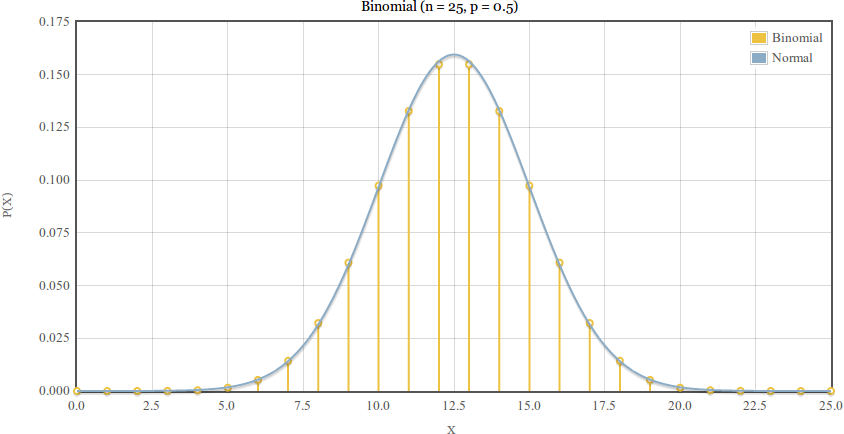
\includegraphics[width=\textwidth]{../images/binomial-normal-1.png}}
    \only<2>{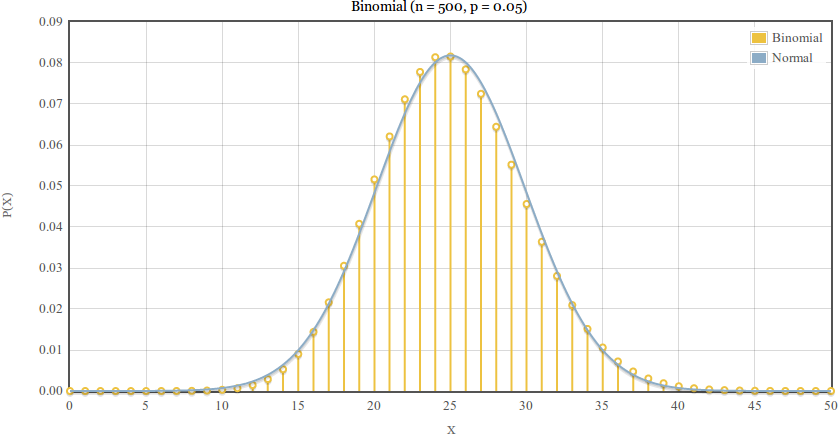
\includegraphics[width=\textwidth]{../images/binomial-normal-2.png}}
  \end{center}
}
\frame{ \frametitle{Introduction}

  However, when $n$ is medium and $p$ is extreme ...

  \begin{center}
    \only<1>{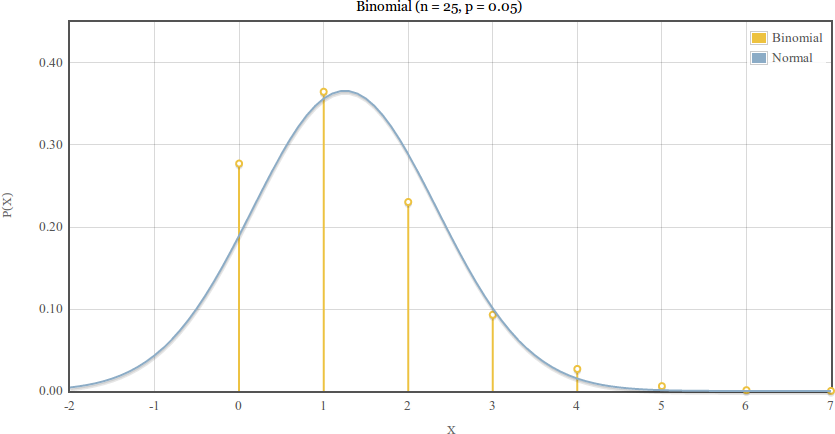
\includegraphics[width=\textwidth]{../images/binomial-normal-sn-1.png}}
    \only<2-3>{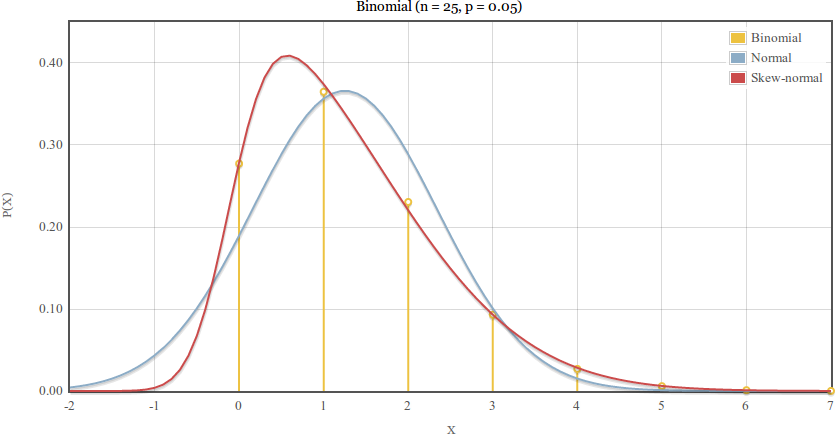
\includegraphics[width=\textwidth]{../images/binomial-normal-sn-2.png}}
    \only<4>{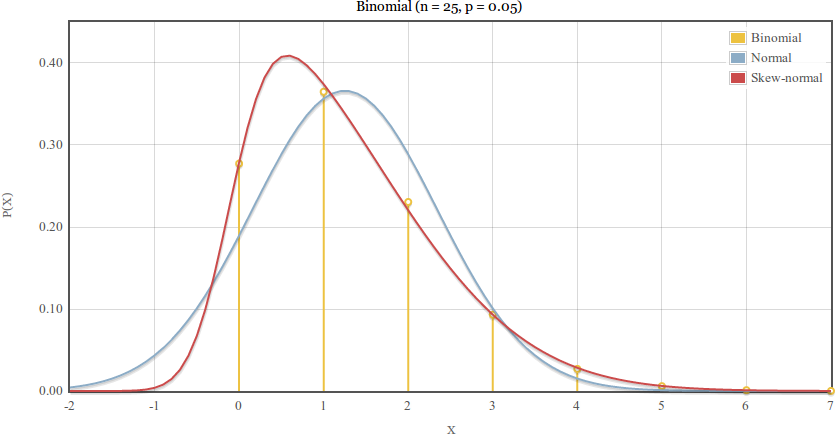
\includegraphics[width=\textwidth]{../images/binomial-normal-sn-3.png}}
  \end{center}

  \only<1>{the binomial is very skewed.}
  \only<2>{the normal approximation doesn't work very well.}
  \only<3->{\textbf{Can we do better?}}
  \only<4>{Introducing ... the skew-normal distribution.}
}

%% Outline
\frame{ \frametitle{Outline}
  What we're going to cover:
  \pause
  \begin{enumerate}[<+->]
    \item Skew-Normal distribution -- basic properties
    \item Method of Moments -- derive an approximation
    \item Accuracy -- compare to the normal approximation
  \end{enumerate}
}

% The Skew-Normal Distribution
\frame{ \frametitle{The Skew-Normal Distribution: Foundations}
  \begin{definition}[Skew-normal]
    Let $Y$ be a skew-normal distribution, with location parameter $\mu \in
    \R$, scale parameter $\sigma > 0$, and shape parameter $\lambda \in \R$.
    Then $Y$ has pdf

    \begin{equation*}
      f(x|\mu, \sigma, \lambda) = \frac2\sigma \cdot \phi \left( \frac{x-\mu}{\sigma} \right) \cdot \Phi \left( \frac{\lambda(x-\mu)}{\sigma} \right), \quad x \in \R,
    \end{equation*}

    where $\phi$ is the standard normal pdf and $\Phi$ is the standard normal
    cdf.

    \vsep
    We write $Y \sim SN(\mu, \sigma, \lambda)$.
  \end{definition}
}
\frame{ \frametitle{The Skew-Normal Distribution: Foundations}
  \begin{lem*}
    If $f_0$ is a one-dimensional probability density function symmetric about
    0, and $G$ is a one-dimensional distribution function such that $G'$ exists
    and is a density symmetric about 0, then

    \begin{equation*}
      f(z) = 2 \cdot f_0(z) \cdot G\{w(z)\} \quad (-\infty < z < \infty)
    \end{equation*}

    is a density function for any odd function $w(\cdot)$. (Lemma 1,
    \citealp{azzalini})
  \end{lem*}
}
\frame{ \frametitle{The Skew-Normal Distribution: Foundations}

  Basic properties:

  \begin{align*}
    E(Y) &= \mu + b \delta \sigma \\
    E(Y^2) &= \mu^2 + 2b \delta \mu \sigma + \sigma^2 \\
    E(Y^3) &= \mu^3 + 3 b \delta \mu^2 \sigma + 3 \mu \sigma^2 + 3 b \delta \sigma^3 - b \delta^3 \sigma^3 \\
    Var(Y) &= \sigma^2 (1 - b^2 \delta^2)
  \end{align*}

  where $b = \sqrt{\frac{2}{\pi}}$ and $\delta = \frac{\lambda}{\sqrt{1 +
  \lambda^2}}$. \citep{pewsey}
}
\frame{ \frametitle{The Skew-Normal Distribution: Foundations}

  What happens when $\lambda=0$?

  \begin{align*}
    f(x|\mu, \sigma, \lambda=0) &= \frac2\sigma \cdot \phi \left( \frac{x-\mu}{\sigma} \right) \cdot \Phi(0) \\
    &= \frac2\sigma \cdot \phi \left( \frac{x-\mu}{\sigma} \right) \cdot 0.5 \\
    &= \frac1\sigma \cdot \phi \left( \frac{x-\mu}{\sigma} \right) \\
    &= \frac{1}{\sqrt{2\pi}\sigma} \;\cdot\; \exp \left( -\frac{(x-\mu)^2}{2\sigma^2} \right),
  \end{align*}

  which is the pdf of the normal distribution ($\mu$, $\sigma$).
}
\frame{ \frametitle{The Skew-Normal Distribution: The Standard Skew-Normal}

  \begin{definition}[Standard skew-normal]
    The $SN(0,1,\lambda)$ distribution is called the standard skew-normal and
    has pdf

    \begin{equation*}
      f_Z(x|\lambda) = 2 \cdot \phi(x) \cdot \Phi (\lambda x), \quad x \in \R.
    \end{equation*}
  \end{definition}

  Similar to the normal and standard normal, $Z = \frac{Y - \mu}{\sigma}$ and $Y
  = \sigma Z + \mu$.
}
\frame{ \frametitle{The Skew-Normal Distribution: The Standard Skew-Normal}

  \begin{property}
    If $Z \sim SN(0, 1, \lambda)$, then $(-Z) \sim SN(0, 1, -\lambda)$.
  \end{property}
  \vsep
  \begin{property}
    If $Z \sim SN(0, 1, \lambda)$, then $Z^2 \sim \chi^2_1$ (chi-square with 1 degree of freedom).
  \end{property}
}
\frame{ \frametitle{The Skew-Normal Distribution}
  \frametitle{The Skew-Normal Distribution: The Standard Skew-Normal}

  \begin{property}
    As $\lambda \to \pm \infty$, \thinspace $SN(0,1,\lambda)$ tends to the half normal distribution, $\pm |N(0,1)|$.
  \end{property}
  \vsep
  \begin{property}
    The moment generating function of $SN(0,1,\lambda)$ is

    \begin{equation*}
      M(t|\lambda) = 2 \cdot \Phi (\delta t) \cdot e^{t^2/2},
    \end{equation*}
    
    where $\delta = \frac{\lambda}{\sqrt{1 + \lambda^2}}$ and $t \in (-\infty, \infty)$.
  \end{property}
}

% Method of Moments

\frame{ \frametitle{Method of Moments: Overview}
  Game plan:
  \begin{enumerate}[<+->]
    \item Find the first three central moments of the binomial and the first
          three central moments of the skew-normal.\\
          \vsep         
          What are central moments?: $E(X)$, $E([X - E(X)]^2)$, $E([X -
          E(X)]^3)$.
    \item Set them equal to each other.
    \item Take $n$ and $p$ to be constants; solve for $\mu$, $\sigma$, and $\lambda$.
  \end{enumerate}
}

%% The Central Moments of the Binomial
\frame{ \frametitle{Method of Moments: Central Moments of the Binomial}
  The first two are easy:
  \begin{align*}
    E(B) &= np \\
    E([B - E(B)]^2) &= Var(B) = np(1-p)
  \end{align*}
}
\frame{ \frametitle{Method of Moments: Central Moments of the Binomial}
  The third one takes some elbow grease.
  
  First we'll need to find $E(B^2)$ and $E(B^3)$.
}
\frame{ \frametitle{Method of Moments: Central Moments of the Binomial}
  \begin{align*}
    E(B^2) &= Var(B) + [E(B)]^2 \\
    &= np(1-p) + n^2p^2 \\
    &= np - np^2 + n^2p^2
  \end{align*}
}
\frame{ \frametitle{Method of Moments: Central Moments of the Binomial}
  We will get $E(B^3)$ via the third factorial moment, E[B(B-1)(B-2)].
}
\frame{ \frametitle{Method of Moments: Central Moments of the Binomial}
  \begin{align*}
    &E[B(B-1)(B-2)] \\
    &= \sum_{x=0}^n x (x-1) (x-2) \cdot \left\{ \binom{n}{x} p^x q^{n-x} \right\} \\
    &= \sum_{x=3}^n x (x-1) (x-2) \cdot \left\{ \binom{n}{x} p^x q^{n-x} \right\} \\
    &= \sum_{x=3}^n x(x-1)(x-2) \cdot \frac{n!}{x!\;(n-x)!} \; p^x q^{n-x} \\
    &= \sum_{x=3}^n \frac{n!}{(x-3)!\;(n-x)!} \; p^x q^{n-x} \\
    &= \sum_{x=3}^n n(n-1)(n-2) p^3 \cdot \frac{(n-3)!}{(x-3)!\;(n-x)!} \; p^{x-3}q^{n-x} \\
  \end{align*}
}
\frame{ \frametitle{Method of Moments: Central Moments of the Binomial}
  Let $y=x-3$; then $x=y+3$, and $x=3$, $x=n \Ra y=0$, $y=n-3$:
  \begin{align*}
    &= \sum_{x=3}^n n(n-1)(n-2) p^3 \cdot \frac{(n-3)!}{(x-3)!\;(n-x)!} \; p^{x-3}q^{n-x} \\
    &= n(n-1)(n-2)p^3 \cdot \sum_{y=0}^{n-3} \frac{(n-3)!}{y!\;(n-(y+3))!} \; p^y q^{n-(y+3)} \\
    &= n(n-1)(n-2)p^3 \cdot \underbrace {\sum_{y=0}^{n-3} \frac{(n-3)!}{y!\;((n-3)-y)!} \; p^y q^{(n-3)-y}}_{\mathclap{\textnormal{[pdf of $Bin(n-3,p)$ summed over its domain] = 1}}} \\
    &= n(n-1)(n-2)p^3 \\
    &= n^3p^3 - 3n^2p^3 + 2np^3
  \end{align*}
}
\frame{ \frametitle{Method of Moments: Central Moments of the Binomial}
  To get $E(B^3)$, we expand the left side of the previous equation:
  \begin{align*}
    &E[B(B-1)(B-2)] \\
    &= E \left[ B^3 - 3B^2 + 2B \right] \\
    &= E(B^3) - 3E(B^2) + 2E(B) \\
    &= E(B^3) - 3(np - np^2 + n^2p^2) + 2np \\
    &= E(B^3) - 3np + 3np^2 - 3n^2p^2 + 2np \\
    &= E(B^3) + 3np^2 - 3n^2p^2 - np
  \end{align*}
}
\frame{ \frametitle{Method of Moments: Central Moments of the Binomial}
  Left side: $E(B^3) + 3np^2 - 3n^2p^2 - np$

  Right side: $n^3p^3 - 3n^2p^3 + 2np^3$

  Set them equal and solve for $E(B^3)$:
  \begin{align*}
    &E(B^3) + 3np^2 - 3n^2p^2 - np = n^3p^3 - 3n^2p^3 + 2np^3 \\
    &\Rightarrow \qquad E(B^3) = n^3p^3 - 3n^2p^3 + 2np^3 - 3np^2 + 3n^2p^2 + np
  \end{align*}
}
\frame{ \frametitle{Method of Moments: Central Moments of the Binomial}
  Now we can (finally!) compute the third central moment:
  \begin{align*}
    &E \left( [B - E(B)]^3 \right) \\
    &= E \left( B^3 - 3B^2 E(B) + 3B [E(B)]^2 - [E(B)]^3 \right) \\
    &= E(B^3) - 3 E(B^2) E(B) + 3 E(B) [E(B)]^2 - [E(B)]^3 \\
    &= E(B^3) - 3 E(B^2) E(B) + 2 [E(B)]^3 \\
    &= (n^3p^3 - 3n^2p^3 + 2np^3 - 3np^2 + 3n^2p^2 + np) \\
    &\quad - 3(np - np^2 + n^2p^2)(np) + 2(np)^3 \\
    &= \cancel{n^3p^3} - \cancel{3n^2p^3} + 2np^3 - 3np^2 + \cancel{3n^2p^2} + np \\
    &\quad - \cancel{3n^2p^2} + \cancel{3n^2p^3} - \cancel{3n^3p^3} + \cancel{2n^3p^3} \\
    &= 2np^3 - 3np^2 + np \\
    &= np(p-1)(2p-1)
  \end{align*}
}
\frame{ \frametitle{Method of Moments: Central Moments of the Binomial}
  Let's restate our results:
  \begin{align*}
    E(B) &= np, \\
    E([B - E(B)]^2) &= np(1-p), \\
    E([B - E(B)]^3) &= np(p-1)(2p-1)
  \end{align*}
}

%% The Central Moments of the Skew-Normal
\frame{ \frametitle{Method of Moments: Central Moments of the Skew-Normal}
  The first and second central moments are the mean and variance.
  \begin{align*}
    E(Y) &= \mu + b \delta \sigma \\
    Var(Y) &= \sigma^2 (1 - b^2 \delta^2)
  \end{align*}
}
\frame{ \frametitle{Method of Moments: Central Moments of the Skew-Normal}
  Again, the third one is a little harder:
  \begin{align*}
    &E([Y - E(Y)]^3) \\
    &= E(Y^3) - 3E(Y^2)E(Y) + 2[E(Y)]^3 \\
    &= (\mu^3 + 3 b \delta \mu^2 \sigma + 3 \mu \sigma^2 + 3 b \delta \sigma^3 - b \delta^3 \sigma^3) \\
    &\quad - 3 (\mu^2 + 2b \delta \mu \sigma + \sigma^2) (\mu + b \delta \sigma) + 2\;(\mu + b \delta \sigma)^3 \\
    &= \cancel{\mu^3} + \cancel{3 b \delta \mu^2 \sigma} + \cancel{3 \mu \sigma^2} + \cancel{3 b \delta \sigma^3} - b \delta^3 \sigma^3 - \cancel{3 \mu^3} - \cancel{3 b \delta \mu^2 \sigma} \\
    &\quad - \cancel{6 b \delta \mu^2 \sigma} - \cancel{6 b^2 \delta^2 \mu \sigma^2} - \cancel{3 \mu \sigma^2} - \cancel{3 b \delta \sigma^3} + \cancel{2 \mu^3} + \cancel{6 b \delta \mu^2 \sigma} \\
    &\quad + \cancel{6 b^2 \delta^2 \mu \sigma^2} + 2 b^3 \delta^3 \sigma^3 \\
    &= 2 b^3 \delta^3 \sigma^3 - b \delta^3 \sigma^3 \\
    &= b \delta^3 \sigma^3 (2b^2 - 1)
  \end{align*}
}
\frame{ \frametitle{Method of Moments: Central Moments of the Skew-Normal}
  Our results, restated:
  \begin{alignat*}{4}
    E(Y) &= \mu + b \delta \sigma \;&=&\; \mu + \sigma \cdot \sqrt{\frac{2}{\pi}} \cdot \frac{\lambda}{\sqrt{1 + \lambda^2}} \\
    E([Y - E(Y)]^2) &= \sigma^2 (1 - b^2 \delta^2) \;&=&\; \sigma^2 \left( 1 - \frac{2}{\pi} \cdot \frac{\lambda^2}{1 + \lambda^2} \right) \\
    E([Y - E(Y)]^3) &= b \delta^3 \sigma^3 (2b^2 - 1) \;&=&\; \sigma^3 \sqrt{\frac{2}{\pi}} \left( \frac{\lambda}{\sqrt{1 + \lambda^2}} \right)^3 \left( \frac{4}{\pi} - 1 \right)
  \end{alignat*}
}

%% Deriving an Approximation
\frame{ \frametitle{Method of Moments: Deriving an Approximation}
  Set the central moments of the binomial equal to the central moments of the skew-normal:
  \begin{subequations}
  \begin{align}
    np &= \mu + \sigma \cdot \sqrt{\frac{2}{\pi}} \cdot \frac{\lambda}{\sqrt{1 + \lambda^2}} \label{eq:first-moment-set} \\
    np(1-p) &= \sigma^2 \left( 1 - \frac{2}{\pi} \cdot \frac{\lambda^2}{1 + \lambda^2} \right) \label{eq:second-moment-set} \\
    np(p-1)(2p-1) &= \sigma^3 \sqrt{\frac{2}{\pi}} \left( \frac{\lambda}{\sqrt{1 + \lambda^2}} \right)^3 \left( \frac{4}{\pi} - 1 \right) \label{eq:third-moment-set}
  \end{align}
  \end{subequations}
}
\frame{ \frametitle{Method of Moments: Deriving an Approximation}
  To get $\lambda$, divide the cube of \eqref{eq:second-moment-set} by the
  square of \eqref{eq:third-moment-set}:
  \begin{align}
    \frac{\sigma^6 \left( 1 - \frac{2}{\pi} \cdot \frac{\lambda^2}{1 + \lambda^2} \right)^3}{\sigma^6 \cdot \frac{2}{\pi} \left( \frac{\lambda}{\sqrt{1 + \lambda^2}} \right)^6 \left(
      \frac{4}{\pi} - 1 \right)^2} &= \frac{n^3p^3(1-p)^3}{n^2p^2(p-1)^2(2p-1)^2} \nonumber \\
    \Rightarrow \quad \frac{\left( 1 - \frac{2}{\pi} \cdot \frac{\lambda^2}{1+\lambda^2} \right)^3}{\frac{2}{\pi} \left( \frac{\lambda^2}{1+\lambda^2} \right)^3 \left( \frac{4}{\pi} - 1
      \right)^2} &= \frac{np(1-p)}{(1-2p)^2} \;. \label{eq:solving-for-lambda}
  \end{align}
}
\frame{ \frametitle{Method of Moments: Deriving an Approximation}
  Equation \eqref{eq:solving-for-lambda} can be solved for $\lambda^2$. Then take
  \begin{equation*}
    \lambda = \textnormal{\{sign of $(1-2p)$\}} \sqrt{\lambda^2}
  \end{equation*}
}
\frame{ \frametitle{Method of Moments: Deriving an Approximation}
  With $\lambda$, solve for $\sigma$ and then $\mu$
  \begin{equation*}
    np(1-p) = \sigma^2 \left( 1 - \frac{2}{\pi} \cdot \frac{\lambda^2}{1 + \lambda^2} \right) \quad\Rightarrow\quad
    \sigma = \sqrt{\frac{np(1-p)}{1 - \frac{2}{\pi} \cdot \frac{\lambda^2}{1 + \lambda^2}}}
  \end{equation*}
  \begin{equation*}
    np = \mu + \sigma \cdot \sqrt{\frac{2}{\pi}} \cdot \frac{\lambda}{\sqrt{1 + \lambda^2}} \quad\Rightarrow\quad
    \mu = np - \sigma \cdot \sqrt{\frac{2}{\pi}} \cdot \frac{\lambda}{\sqrt{1 + \lambda^2}}
  \end{equation*}
}
\frame{ \frametitle{Method of Moments: Deriving an Approximation}
  When $p = 0.5$, $\lambda=0$.
}

%% Restrictions
\frame{ \frametitle{Method of Moments: Restrictions}
  Let $u = \frac{\lambda^2}{1+\lambda^2}$ and $v = 1/u = \frac{1+\lambda^2}{\lambda^2}$.

  Then we can rewrite \eqref{eq:solving-for-lambda}:
  \begin{gather*}
    \frac{\left( 1 - \frac{2}{\pi} \cdot \frac{\lambda^2}{1+\lambda^2} \right)^3}{\frac{2}{\pi} \left( \frac{\lambda^2}{1+\lambda^2} \right)^3 \left( \frac{4}{\pi} - 1 \right)^2} \\
    \vdots \\
    (magic) \\
    \vdots \\
    \left( v - \frac{2}{\pi} \right)^3 \left( \frac{\pi^3}{2(4-\pi)^2} \right) = g(v)
  \end{gather*}
}
\frame{ \frametitle{Method of Moments: Restrictions}
  $g(v)$ is increasing in $v = \frac{1+\lambda^2}{\lambda^2} \geq 1$. Therefore:
  \begin{equation*}
    \min_{v} g(v) = g(1) = \left( 1 - \frac{2}{\pi} \right)^3 \left( \frac{\pi^3}{2(4-\pi)^2} \right) = 1.009524 \approx 1
  \end{equation*}
}
\frame{ \frametitle{Method of Moments: Restrictions}
  To be able to solve \eqref{eq:solving-for-lambda} for $\lambda$, we must have
  \begin{align}
    \textnormal{\{right hand side of \eqref{eq:solving-for-lambda}\}} &\geq \textnormal{\{min of left hand side of \eqref{eq:solving-for-lambda}\}} \nonumber \\
    \frac{np(1-p)}{(1-2p)^2} &\geq 1 \nonumber \\
    np(1-p) &\geq (1-2p)^2. \label{eq:solving-the-restriction}
  \end{align}
}
\frame{ \frametitle{Method of Moments: Restrictions}
  From \eqref{eq:solving-the-restriction}, we can answer two questions:

  Given $p$, what is the least $n$ necessary?
  \begin{equation*}
    n \geq \frac{(1-2p)^2}{p(1-p)}
  \end{equation*}
  Given $n$, what is the range of possible $p$'s?
  \begin{equation*}
   \frac12 - \frac12 \sqrt{\frac{n}{n+4}} \; \leq \; p \; \leq \; \frac12 + \frac12 \sqrt{\frac{n}{n+4}}
  \end{equation*}
}
\frame{ \frametitle{Method of Moments: Restrictions}
  % figures
}

% Demonstrating Improved Accuracy

%% Visual Inspection
\frame{ \frametitle{Demonstrating Improved Accuracy: Visual}
  %figures
}

%% MABS
\frame{ \frametitle{Demonstrating Improved Accuracy: MABS}
  \begin{equation*}
    \textnormal{MABS}(n, p) \eq \max_{k \in \{0, 1,...,n\}} \left| F_{B(n,p)} (k) -  F_{\textnormal{appr}(n,p)}(k + 0.5) \right|
  \end{equation*}
}
\frame{ \frametitle{Demonstrating Improved Accuracy: MABS}
  %figures
}

\frame{
  \frametitle{Resources}
}

\begin{frame}[allowframebreaks]
  \frametitle{Bibliography}
  \nocite{*}
  \bibliography{../bibliography.bib}
  \bibliographystyle{plainnat}
\end{frame}
\end{document}
